\documentclass{article}
\usepackage{CJK}
\usepackage{ctex}
\usepackage{graphicx}
\usepackage{float}
\usepackage[colorlinks,linkcolor=black]{hyperref}
\graphicspath{{pic/}}
\renewcommand{\contentsname}{目录}
\renewcommand{\abstractname}{摘要}
\author{杨铭 - 5130379022}
\title{游戏设计 - 第三次作业报告}
\begin{document}
\maketitle
\tableofcontents
\section{三维模型}
\subsection{工具介绍}
\paragraph{}
下面是我本次作业使用到的工具和一些资源的源
\begin{description}
  \item[操作系统] windows 10
  \item[3D模型编辑] Blender 2.7.7
  \item[模型来源] sketchfab.com
\end{description}
\paragraph{}
我从\href{https://sketchfab.com/models/5f7371056ba148e0a7936014a9b05030}{sketchfab网站}找了一个动漫少女的模型作为本次作业的资源
\subsection{操作流程}
\subsubsection{模型面片简化}
\paragraph{}使用blender自带的修改器\textbf{decimate}可以直接对模型的面片进行简化
\begin{figure}[H]
\begin{minipage}{0.5\linewidth}
  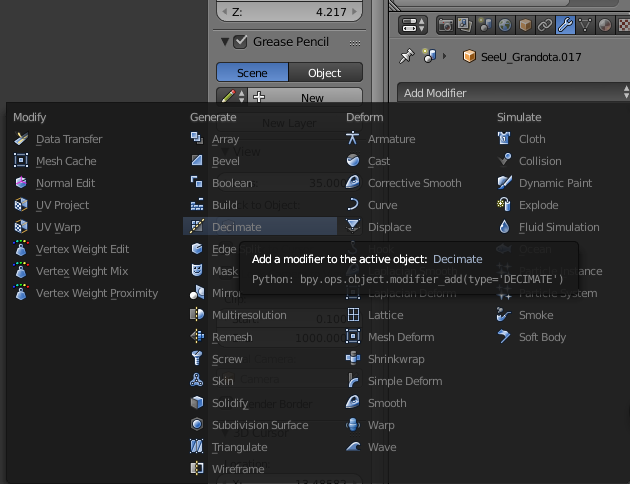
\includegraphics[width=16em]{decimate1.png}\\
  \caption{}\label{1-1}
\end{minipage}
\begin{minipage}{0.5\linewidth}
  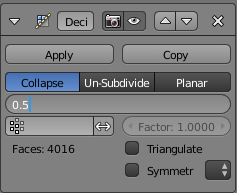
\includegraphics[width=16em]{decimate2.png}\\
  \caption{}\label{1-2}
\end{minipage}
\end{figure}
\paragraph{}
在\textbf{factor}里将简化因素分辨调为0.5、0.2、0.1并且分别应用,即可完成模型简化到50\%、20\%、10\%。
\subsubsection{制作UV贴图}
\paragraph{}
这个部分比前面复杂,由于我选用的模型被合为了一个整体,但在整体的不同部分,使用了不同的材质贴图,所以要先对模型进行分离。
\paragraph{}
进入编辑模式选中模型,按\textbf{P}键呼出\textbf{Separate}菜单,选择\textbf{By Material}选项对模型按照材质分离。
完成后模型被分为了10个部分,为了减少工作量,我选择了面片较多的部分做UV拆分和贴图烘焙
\paragraph{}
导入高模,将其分离并将对应部分留下,其余部分设置为不可见
\begin{figure}[H]
  \centering
  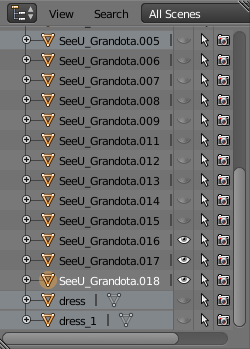
\includegraphics[width=18em]{setting.png}\\
  \caption{物件选项}\label{1-3}
\end{figure}
\paragraph{}
然后选中低模,进入编辑模式,并设置分割线,并新建一个图片保存UV拆分
\begin{figure}
  \centering
  % Requires \usepackage{graphicx}
  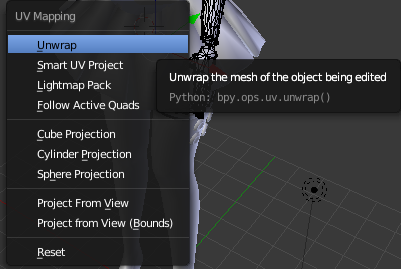
\includegraphics[width=18em]{unwrap.png}\\
  \caption{}\label{1-4}
\end{figure}
\paragraph{}
最后将两个模型重合放置,按照先高模后低模的次序选中两个并进行烘焙即可。注意要将烘焙的模式选为Normals。
\subsection{结果展示}
\paragraph{}
烘焙部分截图如下
\begin{figure}[H]
  \centering
  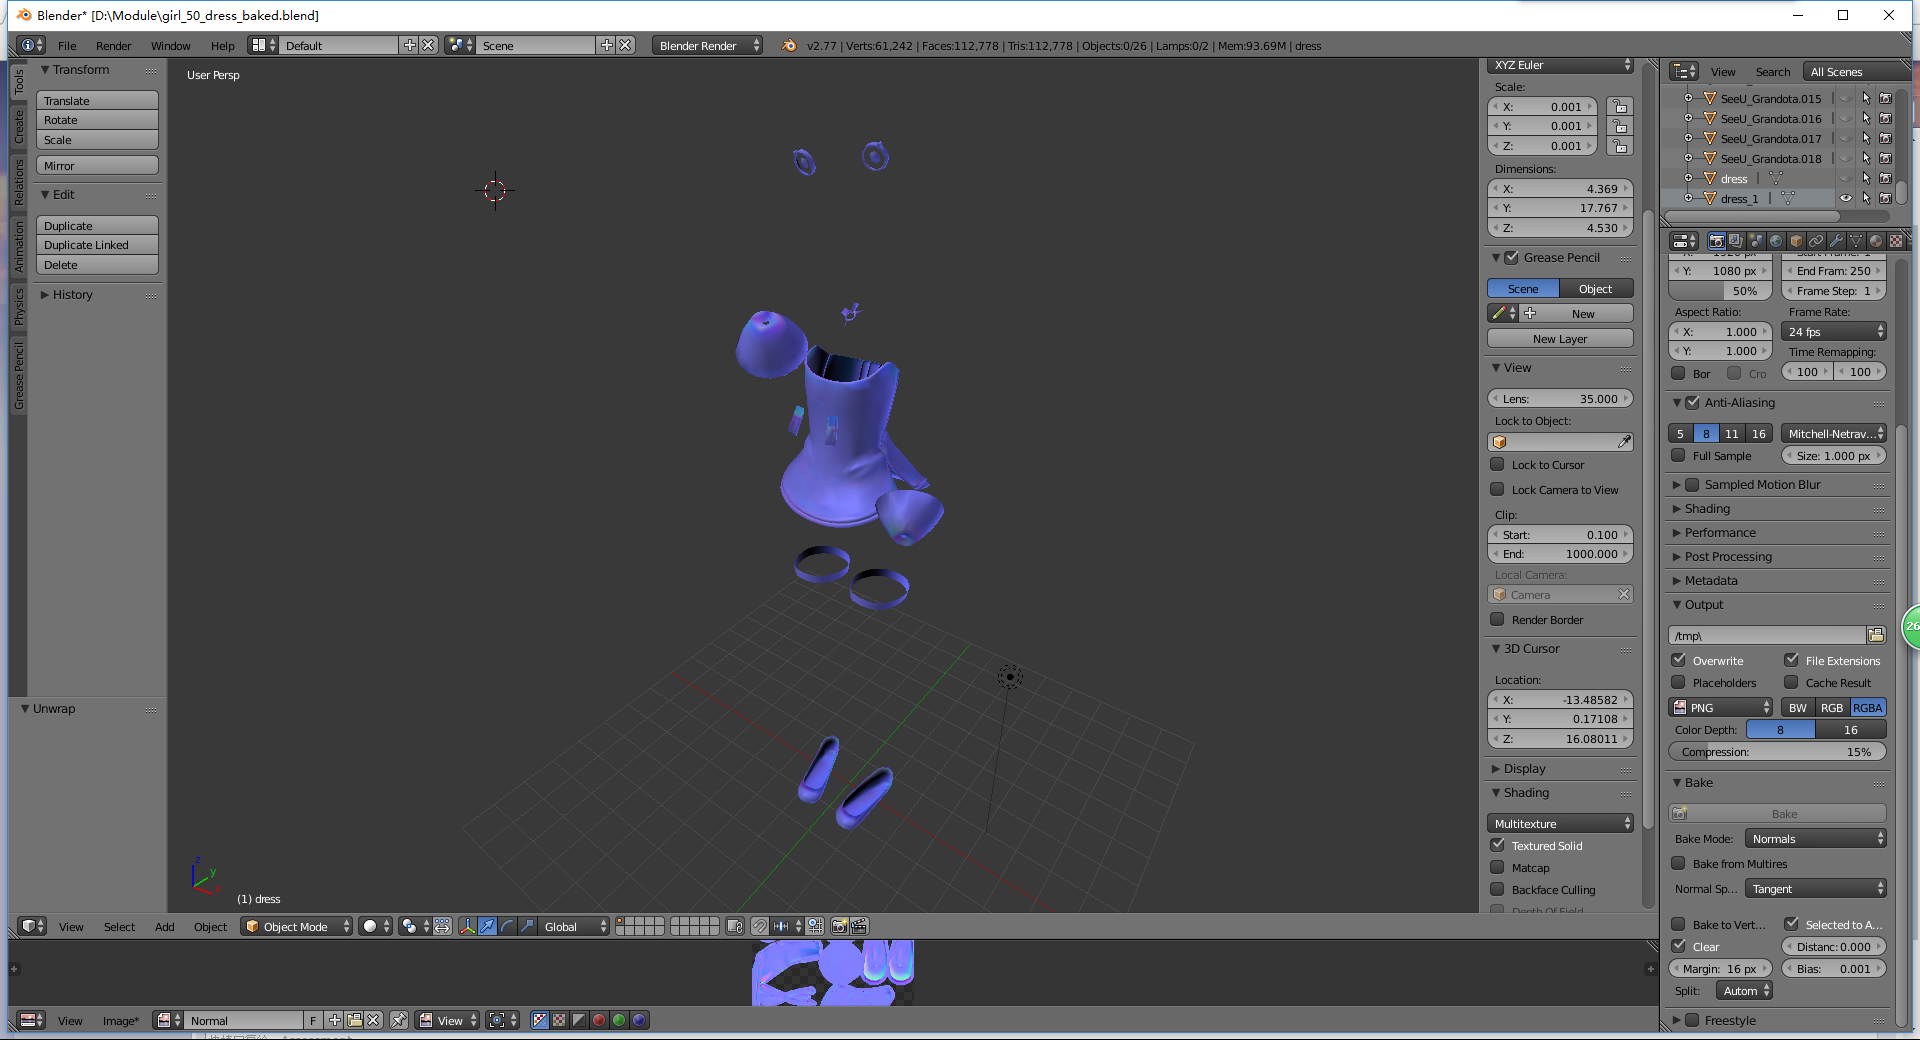
\includegraphics[width=24em]{baking.png}\\
  \caption{}\label{1-5}
  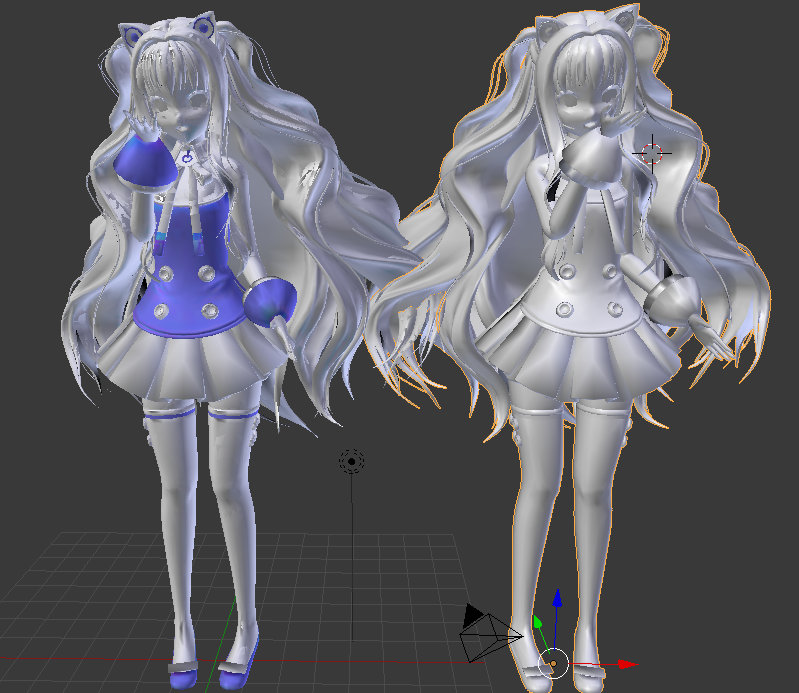
\includegraphics[width=24em]{result.png}\\
  \caption{}\label{1-5}
\end{figure}
\newpage
\section{VR制作}
\paragraph{}
这一部分按照\href{http://www.sitepoint.com/building-a-google-cardboard-vr-app-in-unity/}{教程}一步步来就可以了。需要注意的是导入自己的模型时需要调节一下大小,位置和角度,让模型能较好地处在镜头中心的位置
\begin{figure}[H]
  \centering
  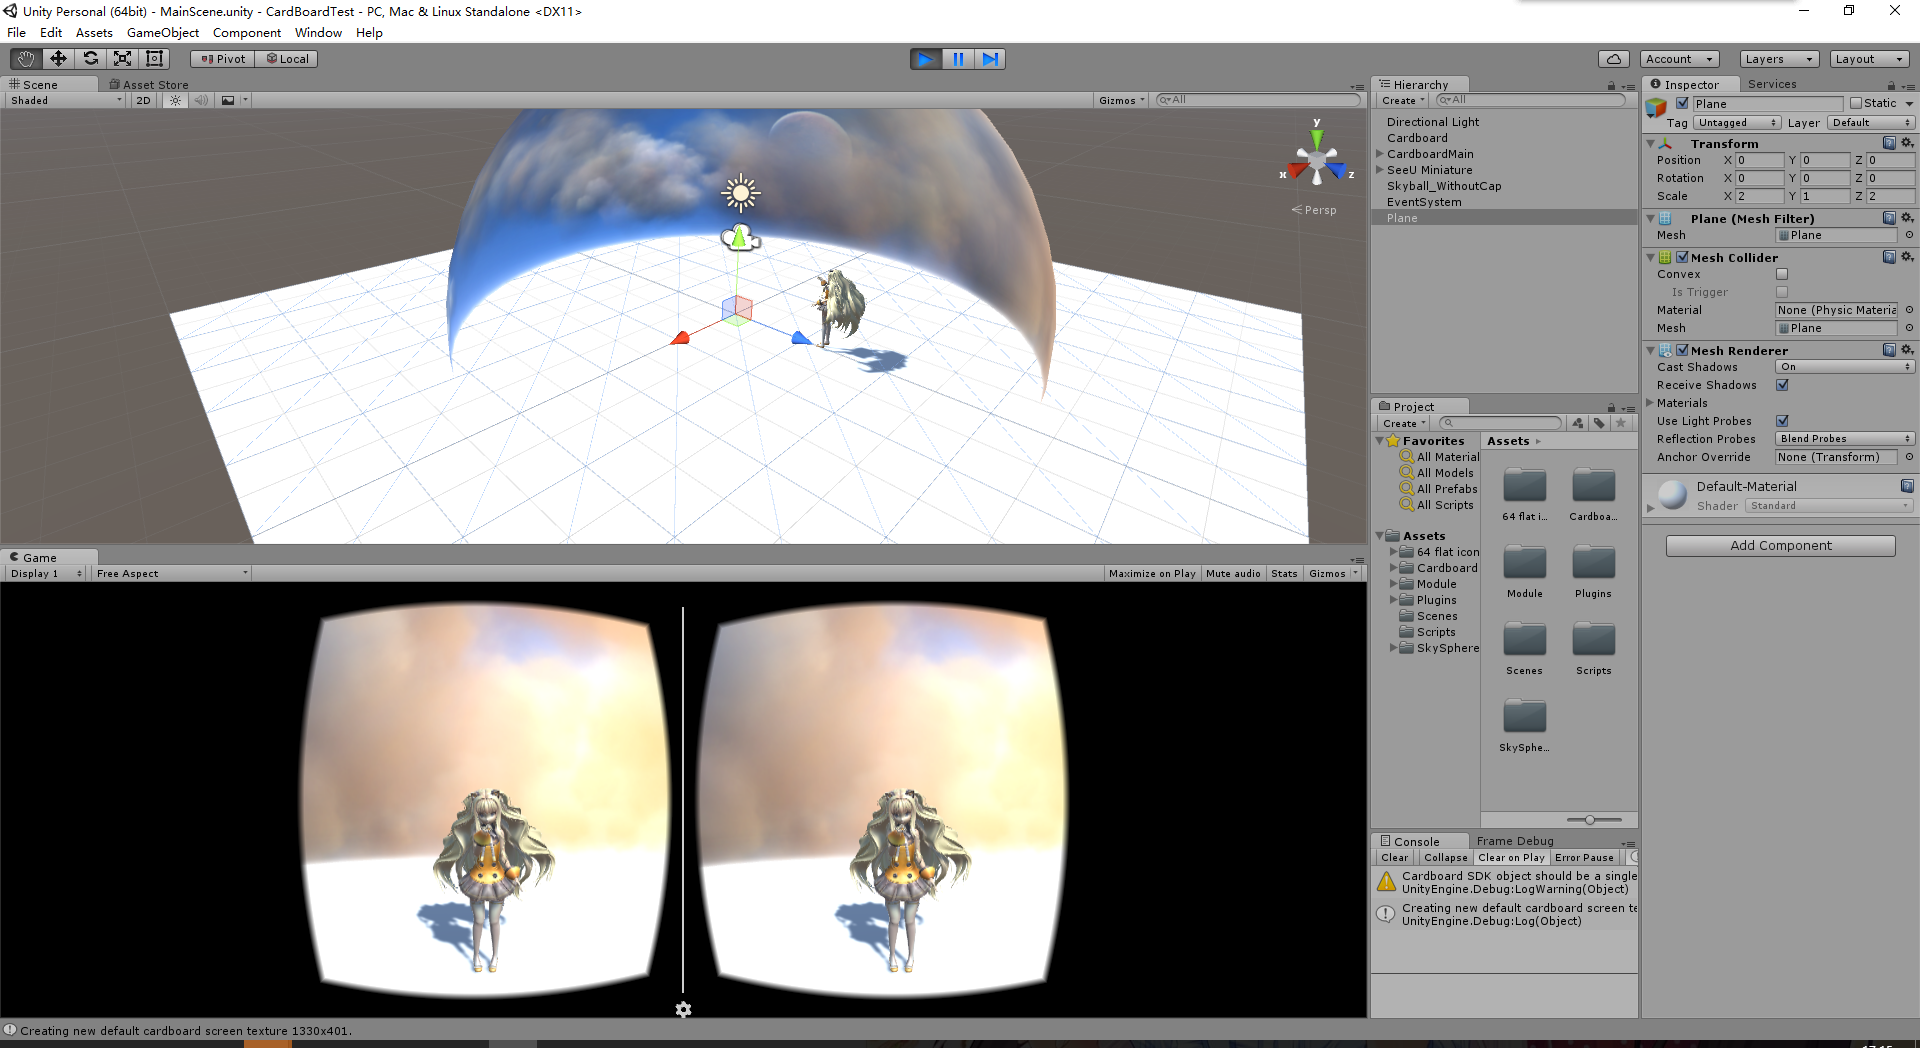
\includegraphics[width=36em]{unity.png}\\
  \caption{}\label{2-1}
\end{figure}
\section{提交说明}
\paragraph{}
因为模型较大,我没有提交导入到Unity工程中的原版.dae模型,提交了简化后的三个.blend文件和一个制作了UV图和纹理烘培的50\%精度与原模型对比.blend文件,需要使用blender打开
\end{document}
